% MATH 201 Lab notes (c) by Carlos Contreras And Philippe Gaudreau
% MATH 201 Lab notes is licensed under a 
% Creative Commons Attribution 4.0 International license.
% CC BY 4.0

% You should have received a copy of the license along with this
% work. If not, see <http://creativecommons.org/licenses/by/4.0/>.

\documentclass[11pt]{article}
% MATH 201 Lab notes (c) by Carlos Contreras And Philippe Gaudreau
% MATH 201 Lab notes is licensed under a 
% Creative Commons Attribution 4.0 International license.
% CC BY 4.0

% You should have received a copy of the license along with this
% work. If not, see <http://creativecommons.org/licenses/by/4.0/>.

%% libraries
\usepackage[utf8x]{inputenc}
\usepackage{xcolor}
\usepackage[left=1.5cm,right=1.5cm,top=2.0cm,bottom=1.5cm,headheight=110pt]{geometry}
\usepackage{amsmath}
\usepackage{amssymb}
\usepackage{graphicx}
\usepackage{xifthen}
\usepackage{sverb}
\usepackage{fancyhdr}
\usepackage{mdframed}
\usepackage{textcomp}

%%%%%%%%%%%%%%%%%%%%%%%%%%%%%%%%%%%%%%%%%%%%%%%%%%%%%%%%%%%%%%%%%%%%%%%
% PDF compiling
\usepackage{ifpdf}
\ifpdf %
        \DeclareGraphicsExtensions{.pdf}%
\else %
        \DeclareGraphicsExtensions{.eps,.ps}%
\fi

%%%%%%%%%%%%%%%%%%%%%%%%%%%%%%%%%%%%%%%%%%%%%%%%%%%%%%%%%%%%%%%%%%%%%%%
% Figures path
\graphicspath{{figures/}}

%%%%%%%%%%%%%%%%%%%%%%%%%%%%%%%%%%%%%%%%%%%%%%%%%%%%%%%%%%%%%%%%%%%%%%%
% Problem counter
\newcounter{Problem}
\setcounter{Problem}{0}

%%%%%%%%%%%%%%%%%%%%%%%%%%%%%%%%%%%%%%%%%%%%%%%%%%%%%%%%%%%%%%%%%%%%%%%
% Definitions
\def\LabSolutions{\clearpage \newpage \begin{center} {\Large \it Solutions} \end{center} \setcounter{Problem}{0}}
\def\QuizSolutions{\newpage \begin{center} {\Large \it Solutions} \end{center} \setcounter{Problem}{0}}
\def\degree{\textdegree}
\def\grade#1{\begin{flushright} {\small [#1]}\\ \end{flushright} \vspace{-10pt}}
\def\codecolor{red!50!black}
\def\code#1{\textcolor{\codecolor}{\tt #1}}
\def\examname#1{%
                \ifnum\value{page}>1%
                    \newpage%
                \else%
                    \vspace*{5pt}%
                \fi%
                \large \textbf{#1} \setcounter{Problem}{0}\vspace{10pt}}
\def\topic#1{\par\needspace{2\baselineskip} \noindent \textsl{\footnotesize #1}}

 
%%%%%%%%%%%%%%%%%%%%%%%%%%%%%%%%%%%%%%%%%%%%%%%%%%%%%%%%%%%%%%%%%%%%%%%
% Environments
\newenvironment{problem}%
     {\stepcounter{Problem}%
      \begin{list}{\textbf{\arabic{Problem}}.~}{}%
      \item}%
     {\end{list}\vspace*{5pt}}

\newenvironment{solution}%
     {\indent \textit{Solution} \newline}%
     {\begin{flushright}$\blacksquare$\end{flushright}}

\newenvironment{preamble}%
     {\vspace*{1em}\begin{mdframed}[leftmargin=1cm,rightmargin=1cm]}%
     {\end{mdframed}\vspace*{1em}}

\newenvironment{multchoice}%
     {\begin{enumerate} \addtolength{\leftskip}{2em} \renewcommand{\labelenumi}{(\alph{enumi})}}
     {\end{enumerate}}

\newenvironment{formulaitem}%
     {\setlength{\leftmargini}{1.5em}\begin{itemize}%
      \setlength\itemindent{-\itemindent}%
      \renewcommand{\labelitemi}{$\rightarrow$}}%
     {\end{itemize}}


%%%%%%%%%%%%%%%%%%%%%%%%%%%%%%%%%%%%%%%%%%%%%%%%%%%%%%%%%%%%%%%%%%%%%%%
% New theorems
\newtheorem{theorem}{Theorem}


\makeatletter

%%%%%%%%%%%%%%%%%%%%%%%%%%%%%%%%%%%%%%%%%%%%%%%%%%%%%%%%%%%%%%%%%%%%%%%
%% New commands
\newcommand*{\course}[1]{\gdef\@course{#1}}
\newcommand*{\coursecode}[1]{\gdef\@coursecode{#1}}
\newcommand*{\term}[1]{\gdef\@term{#1}}
\newcommand*{\instructor}[1]{\gdef\@instructor{#1}}
\newcommand*{\lqnumber}[1]{\gdef\@lqnumber{#1}}
\newcommand*{\labtitle}[1]{\gdef\@labtitle{#1}}
\newcommand*{\quizversion}[1]{\gdef\@quizversion{#1}}
\newcommand*{\probleminfo}[1]{\noindent \textsl{\footnotesize #1}}

% Title header for labs
\newcommand\makelabtitle{%
  \begin{flushleft}%
  {\scshape \@coursecode~\@course~-- University of Alberta}\\%
  {\scshape \@term~-- Labs -- \@instructor}\\%
  {\scshape Authors: Carlos Contreras and Philippe Gaudreau}%
  \end{flushleft}%
  \begin{center}%
  {\Large \bf \@lqnumber:~\@labtitle}%
  \end{center}%
  \thispagestyle{empty}%
  \global\let\@course\@empty%
  \global\let\@labtitle\@empty%
}

% Title header for quizzes
\newcommand\makequiztitle{%
  \begin{flushleft}%
  {\scshape \@coursecode~\@course~-- University of Alberta}\\%
  {\scshape \@term~-- Labs -- \@instructor}\\%
  \end{flushleft}%
  \begin{center}%
  {\Large \bf \@lqnumber} \marginpar{\tiny\tt [\@quizversion]}%
  \end{center}%
  \thispagestyle{empty}%
  \global\let\@course\@empty%
  \global\let\@quizversion\@empty%
}

%%%%%%%%%%%%%%%%%%%%%%%%%%%%%%%%%%%%%%%%%%%%%%%%%%%%%%%%%%%%%%%%%%%%%%%
% Fancy header package
\fancyhead[L]{\small {\scshape \@coursecode~-- \@lqnumber~-- \@term~-- \@instructor}}
\pagestyle{fancy}

\makeatother


\usepackage{hyperref}
\usepackage{cancel}


\begin{document}

\course{Differential Equations}
\coursecode{MATH 201}
\term{Winter 2018}
\instructor{Carlos Contreras}
\lqnumber{Lab 4}
\labtitle{Mecanical vibrations}
\makelabtitle



\begin{problem}
{\bf Pendulum Equation.} Derive the pendulum equation $ m l^2 \theta^{\prime \prime}(t) = -l m g \sin(\theta(t))$.
\end{problem}


\begin{problem}
\textbf{Mass-Spring Equation.} \\
A 2-Kg mass is attached to a spring with stiffness $k = 50$N/m. The mass is displaced $1/4$ m to the left of the equilibrium point and given a velocity of $1$m/sec to the left. Neglecting damping, find the equation of motion of the mass along with the amplitude, period, phase and frequency. How long after release does the mass pass through the equilibrium position?
\end{problem}


\begin{problem}
\textbf{Mass and spring with non-zero forcing.} \\
An 8-Kg mass is attached to a spring hanging from the ceiling and allowed to come to rest. Assume that the spring constant is 40 N/m and the damping constant is 3 N-sec/m. At time $t=0$, an external force of $2\sin(2t +\pi/4)N$ is applied to the system. Determine the amplitude and frequency of the steady-state solution.
\end{problem}


\begin{problem}
{\bf Resonance.} Solve the initial value problem,
\begin{equation*}
\dfrac{{\rm d}^2 y}{{\rm d} t^2} + 9y = 2 \cos(3t), \quad y(0) =1 , y^{\prime}(0) =0.
\end{equation*}
\end{problem}








%%%%%%%%%%%%%%%%%%%%%%%%%%%%%%%%%%%%%%%%%%%%%%%%%%%%%%%%%%%%%%%%%%%%%%%%%%%%%%%%%%%%%%%%%%%%%%%%%%%



\LabSolutions




Theory and problems from: Nagel, Saff \& Sneider, \textit{Fundamentals of Differential Equations}, Eighth Edition, Adisson--Wesley.



\begin{problem}
{\bf Pendulum Equation.} Derive the pendulum equation $ m l^2 \theta^{\prime \prime}(t) = -l m g \sin(\theta(t))$.
\end{problem}

\begin{solution}
To derive the pendulum equation $ m l^2 \theta^{\prime \prime}(t) = -l m g \sin(\theta(t))$, complete the following steps.

{\bf (a)} The \textit{angular momentum} of the pendulum mass $m$ measured about the support $O$ in Figure 4.18 on page 210 of your textbook is given by the product of the "lever arm" length $l$ and the component of the vector momentum $mv$ perpendicular to the lever arm. Show that this gives:

\begin{equation*}
{\rm angular \, \, momentum} = ml^2 \dfrac{{\rm d} \theta}{{\rm d} t}
\end{equation*}

Remember the relation between linear velocity, the radius of an object and its angular velocity :

\begin{equation*}
{\bf v} = r \boldsymbol \omega.
\end{equation*}
In our case the angular velocity is given by $\dfrac{{\rm d} \theta}{{\rm d} t}$ and the radius $r=l$. In addition, we know that the angular velocity vector is always perpendicular to the linear velocity vector in this case.

Hence, we have:

\begin{equation*}
{\rm angular \, \, momentum} =  l \left(ml\dfrac{{\rm d} \theta}{{\rm d} t}\right) =  ml^2 \dfrac{{\rm d} \theta}{{\rm d} t}
\end{equation*}

{\bf (b)} The \textit{torque} produced by gravity equals the product of the lever arm length $l$ and the component of gravitational (vector) force $m {\bf g}$ perpendicular to the lever arm. Show that this gives:

\begin{equation*}
{\rm torque} = -lmg\sin(\theta)
\end{equation*}

See the picture in the lab.

{\bf (c)} Now use Newton's law of rotational motion to deduce the pendulum equation.

Newton's law of rotational motion states that the torque is equal to the rate of change of the angular velocity. Hence,

\begin{equation*}
-lmg\sin(\theta) = \dfrac{{\rm d} }{{\rm d} t} \left( ml^2 \dfrac{{\rm d} \theta}{{\rm d} t} \right) =ml^2 \dfrac{{\rm d^2} \theta}{{\rm d} t^2}
\end{equation*}

Simplifying, we obtain:

\begin{equation} \label{formula: pendulum equation}
\theta^{\prime \prime} + \left(\dfrac{g}{l} \right) \sin(\theta) = 0
\end{equation}
This is a non-linear equation, and we don't have the tools to solve such an equation. However, let's consider a special case.

We know from the Taylor series of $\sin(\theta)$, that for small angles:

\begin{equation*}
\sin(\theta) \approx \theta.
\end{equation*}

Hence, for small angles, \eqref{formula: pendulum equation} becomes:

\begin{equation} \label{formula: pendulum equation small angles}
\theta^{\prime \prime} + \left(\dfrac{g}{l} \right) \theta = 0
\end{equation}
This is a constant coefficient second order ODE. We know how to solve this equation using the auxiliary equation. In this case, we have:

\begin{equation*}
r^2 + \left(\dfrac{g}{l} \right) = 0, \quad \Rightarrow \quad r = 0 \pm i \sqrt{\dfrac{g}{l} }
\end{equation*}
If we let  $ \omega = \sqrt{\dfrac{g}{l} }$, we have the general solution:

\begin{equation*}
\theta(t) = C_{1} \cos(\omega t) + C_{2} \sin(\omega t).
\end{equation*}

We have two arbitrary constants in our solutions. Can we set up two initial conditions to obtain an exact solution. If we set up our mass at an angle of $\theta_{o}$ at time $t=0$, and give it no initial velocity, we can write:

\begin{eqnarray*}
\theta(0) & = & \theta_{o}, \\
\theta^{\prime}(0) & = & 0.
\end{eqnarray*}

Applying these two conditions, we find:

\begin{eqnarray*}
C_{1} & = & \theta_{o}, \\
C_{2} & = & 0.
\end{eqnarray*}
Hence the exact solution is given by:

\begin{equation*}
\theta(t) = \theta_{o} \cos(\omega t).
\end{equation*}
\end{solution}




\begin{problem}
\textbf{Mass-Spring Equation.} \\
A 2-Kg mass is attached to a spring with stiffness $k = 50$N/m. The mass is displaced $1/4$ m to the left of the equilibrium point and given a velocity of $1$m/sec to the left. Neglecting damping, find the equation of motion of the mass along with the amplitude, period, phase and frequency. How long after release does the mass pass through the equilibrium position?
\end{problem}
\begin{solution}
 Let $x(t)$ denote the position of the mass on the spring at time $t$. In summary, we have the following data:

\begin{eqnarray*}
m & = & 2Kg \\
k & = & 50N/m \\
x(0) & = & -1/4 m \\
x^{\prime}(0) & = & -1 m/s \\
\end{eqnarray*}

Newton's second law state that sum of all forces is equal to the change in momentum. That is:

\begin{equation*}
\sum {\bf F} = m {\bf a} = m \dfrac{{\rm d}^2 x(t)}{{\rm d} t^2}
\end{equation*}
In our case, the only force acting on our spring is given by Hook's law which states:

\begin{equation*}
\sum {\bf F} = -k x(t).
\end{equation*}
Putting all of this together, we have:

\begin{equation*}
m \dfrac{{\rm d}^2 x(t)}{{\rm d} t^2} = -k x(t), \quad x(0) = -1/4 , \quad x^{\prime}(0) = -1.
\end{equation*}

\begin{equation*}
 \dfrac{{\rm d}^2 x(t)}{{\rm d} t^2} +\left( \dfrac{k}{m} \right) x(t), \quad x(0) = -1/4 , \quad x^{\prime}(0) = -1.
\end{equation*}

This is a second degree ODE with constant coefficients! The auxiliary equation is given by:
\begin{equation*}
 r^2 +\left( \dfrac{k}{m} \right) =0, \quad \Rightarrow \quad r = 0 \pm i \sqrt{\dfrac{k}{m}} = 0 \pm i \sqrt{\dfrac{50}{2}} = 0 \pm 5 i
\end{equation*}

\begin{eqnarray*}
x(t) & = & C_{1} \cos(5 t) + C_{2} \sin(5 t), \\
x^{\prime}(t) & = & - 5 C_{1} \sin(5 t) + 5 C_{2} \cos(5 t).
\end{eqnarray*}
From this we can see that angular frequency of our mass is $\omega = 5$ rad/s.
Setting $ t=0 $, we obtain:
\begin{eqnarray*}
-1/4 & = & C_{1}  \\
-1 & = &  5 C_{2} .
\end{eqnarray*}
Hence, the equation of motion is given by:
\begin{equation*}
x(t) =  -\dfrac{1}{4} \cos(5 t) -\dfrac{1}{5} \sin(5 t)
\end{equation*}

The amplitude of our system can be found by:

\begin{equation*}
A =  \sqrt{\left(C_{1}\right)^2 + \left(C_{2}\right)^2} = \sqrt{\left(-\dfrac{1}{4}\right)^2 + \left(-\dfrac{1}{5}\right)^2} = \dfrac{\sqrt{41}}{20} \approx 0.32017 m
\end{equation*}

The phase of our system is given by:

\begin{equation*}
\tan(\phi) =  \dfrac{C_{2}}{C_{1}} = \dfrac{-\dfrac{1}{5}}{-\dfrac{1}{4}} = \dfrac{4}{5}, \quad \Rightarrow \quad \phi = \arctan(5/4) - \pi \approx -2.2455 rad
\end{equation*}

With these, I can rewrite my equation of motion in the following way:

\begin{equation*}
x(t) =  A \sin ( 5t + \phi)
\end{equation*}

The period of our system is inversely proportional to the angular frequency, that is:

\begin{equation*}
T =  \dfrac{2\pi}{\omega} = \dfrac{2\pi}{5} \approx 1.2566s.
\end{equation*}
The frequency is given by the inverse of the period.

\begin{equation*}
f =  \dfrac{1}{T} = \dfrac{5}{2\pi} \approx 0.79578s^{-1}.
\end{equation*}
To find the first time the mass will cross the equilibrium position,  we have to isolate for $t$ in this equation.

\begin{equation*}
0 =  A \sin ( 5t + \phi) \quad \Rightarrow \quad 5t + \phi =0 \quad \Rightarrow \quad t  = -\dfrac{\phi}{5} = \dfrac{\pi - \arctan(5/4)}{5} \approx 0.44911s.
\end{equation*}
\end{solution}





\begin{problem}
\textbf{Mass and spring with non-zero forcing.} \\
An 8-Kg mass is attached to a spring hanging from the ceiling and allowed to come to rest. Assume that the spring constant is 40 N/m and the damping constant is 3 N-sec/m. At time $t=0$, an external force of $2\sin(2t +\pi/4)N$ is applied to the system. Determine the amplitude and frequency of the steady-state solution.
\end{problem}
\begin{solution}
The equation governing this motion is $my''+by'+ky=F_{\text{ext}}$, with $m=8$Kg, $b=3$N sec/m, and $k=40$ N/m (every constant is in the same system). The roots of the auxiliary equation are
\[r=\frac{-3\pm \sqrt{9-4\cdot8\cdot 40}}{16}=\alpha \pm i \beta,\]
with $\alpha < 0$. We don't need to compute $\beta$ since this is an underdamped motion and the homogeneous solution
\[y_{h}(t)=e^{\alpha t}(C_{1}\cos(\beta t) +C_{2}\sin(\beta t)),\]
decays exponentially. Thus, the steady-state solution (long-term) is the particular solution. Since $0+i2$ is not a root of the auxiliary equation, then, based on the RHS
\[F_{\text{ext}}=2\sin(2t +\pi/4)=+2\sin(\pi/4)\cos(2t)+2\cos(\pi/4)\sin(2t))=\sqrt{2}\cos(2t)+\sqrt{2}\sin(2t),\]
the best guess for the particular solution is,
\begin{eqnarray*}
y_{p}(t) & = & A \cos(2t) + B \sin(2t) ,\\
y_{p}^{\prime}(t) &= &-2A \sin(2t) + 2B \cos(2t) ,\\
y_{p}^{\prime \prime}(t) &= & -4A \cos(2t) - 4B \sin(2t).
\end{eqnarray*}
Substituting our guess into the equation, we obtain the following system
\begin{equation*}\left\{
\begin{array}{cc}
8A + 6B &=\sqrt{2}\\
-6A + 8B &=\sqrt{2}
\end{array}\right. ,
\end{equation*}
which have solution $A=\frac{\sqrt{2}}{50}$ and $B=\frac{7\sqrt{2}}{50}$.
Hence, the steady-state solution is $$y_{\text{st}}(t)\approx y_{p}(t) = \frac{\sqrt{2}}{50}\cos(2t)+ \frac{7\sqrt{2}}{50}\sin(2t),$$
with amplitude and frequency 
\[\boxed{A=\sqrt{C_{1}^{2}+C_{2}^{2}}=\sqrt{\frac{2}{50^{2}}+\frac{49\cdot 2}{50^{2}}}=\frac{1}{5}\text{m}}, \qquad \boxed{f=\frac{\omega}{2\pi}=\frac{2}{2\pi}=\frac{1}{\pi}\text{sec}^{-1}}.\]
\end{solution}





\begin{problem}
{\bf Resonance.} Solve the initial value problem,
\begin{equation*}
\dfrac{{\rm d}^2 y}{{\rm d} t^2} + 9y = 2 \cos(3t), \quad y(0) =1 , y^{\prime}(0) =0.
\end{equation*}
\end{problem}
\begin{solution}
The auxiliary equation for this equation is given by:

\begin{equation*}
r^2 + 9 =0 \quad \Rightarrow \quad r = 0 \pm 3 i
\end{equation*}

Hence:

\begin{equation*}
y_{h}(t) = C_{1} \cos(3 t) + C_{2} \sin(3 t).
\end{equation*}

Let's use the method of variation of parameters to solve for the particular solution:

We try the solution:

\begin{equation*}
y_{p}(t) = C_{1}(t) \cos(3 t) + C_{2}(t) \sin(3 t),
\end{equation*}
where $C_{1}(t)$ and $ C_{2}(t)$ are found using the given formulas from variation of parameters methods.

The Wronskian of these two solutions is:

\begin{equation*}
W[y_{1},y_{2}](t) = \left| \begin{array}{cc} \cos(3 t) & \sin(3 t)\\
-3\sin(3 t) & 3\cos(3 t) \end{array} \right| = 3 \cos^{2}(3 t) + 3\sin^{2}(3 t) = 3;
\end{equation*}

We can find the coefficients $C_{1}(t)$ and $C_{2}(t)$ using  the formulas shown in Lab $\# 4$ with $g(t) = 2 \cos(3t)$.
Hence:

\begin{eqnarray*}
C_{1}(t) & = & - \int \dfrac{g(t) y_{2}(t)}{W[y_{1},y_{2}](t)} {\rm d} t \\
& = & - \int \dfrac{2 \cos(3t)\sin(3t) }{3} {\rm d} t \\
& = & - \int \dfrac{\sin(6t) }{3} {\rm d} t \\
& = & \dfrac{\cos(6t) }{18}
\end{eqnarray*}

\begin{eqnarray*}
C_{2}(t) & = &  \int \dfrac{g(t) y_{1}(t)}{W[y_{1},y_{2}](t)} {\rm d} t \\
& = &  \int \dfrac{2\cos(3t)^2}{3} {\rm d} t \\
& = & \int \dfrac{1+\cos(6t)}{3} {\rm d} t \\
& = & \dfrac{t}{3}+ \dfrac{\sin(6t)}{18}  \\
\end{eqnarray*}

Putting all these results together, we obtain our particular solution:
\begin{eqnarray*}
y_{p}(x) & = & \dfrac{\cos(6t) \cos(3t) }{18} + \dfrac{t}{3} \sin(3t) + \dfrac{\sin(6t) \sin(3t) }{18} \\
          & = & \dfrac{\cos(6t-3t)}{18} + \dfrac{t}{3} \sin(3t)\\
          & = & \dfrac{\cos(3t)}{18} + \dfrac{t}{3} \sin(3t)\\
          & = & \dfrac{t}{3} \sin(3t),\\
\end{eqnarray*}
since $\dfrac{\cos(3t)}{18}$ is part of the homogeneous solution. The general solution is then given by:

\begin{equation}
y(t) = C_{1} \cos(3 t) + C_{2} \sin(3 t) + \dfrac{t}{3} \sin(3t)
\end{equation}
Solving for the constant $C_{1}$ and $C_{2}$ with the initial conditions, we have:

\begin{eqnarray}
C_{1} & = & 1\\
C_{2} & = & 0\\
\end{eqnarray}
Hence the exact solution is given by:
\begin{equation}
y(t) = \cos(3 t)+ \dfrac{t}{3} \sin(3t).
\end{equation}
The plot of the solution is given in the following figure.
\begin{figure}[htb]
\begin{center}
\begin{tabular}{cc} 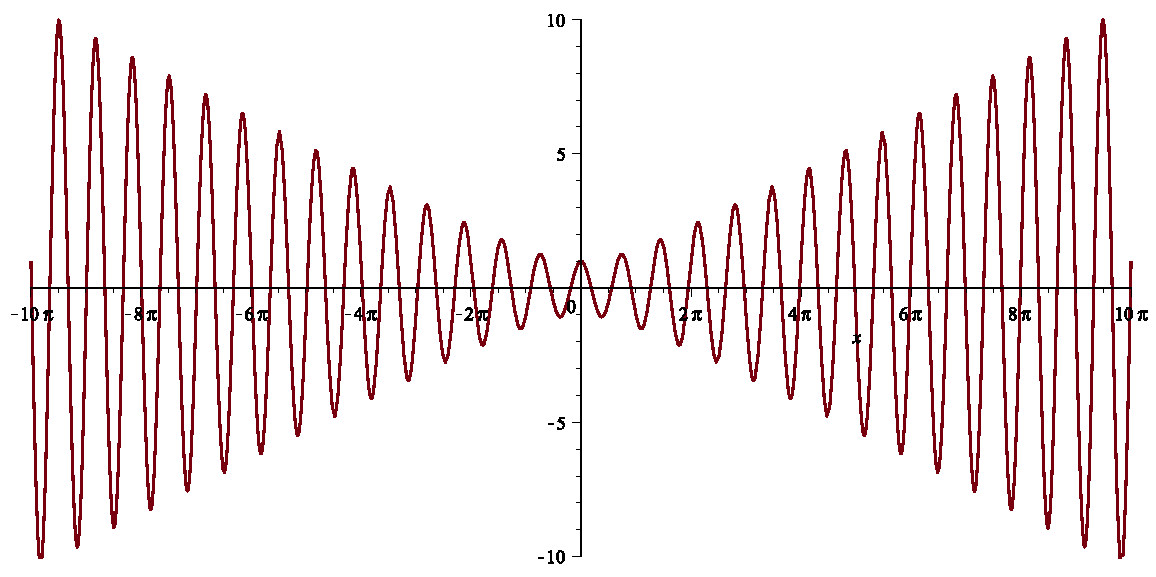
\includegraphics[width=0.7\textwidth]{resonance} \\
\end{tabular}
\end{center}
\end{figure}
\end{solution}





\end{document}
